%!TEX root = ..\..\dissertation.tex
\section{Platform Development Through The Four Loops of Concern}\label{sec:FLC}
\cref{paper:MCPC2017} is entitled~\citetitle{SorensenMCPC2017}, written for and presented at the 9th Mass Customization \& Personalization Conference (MCPC2017) in 2017.
It relates to and addresses \cref{resq1} by answering the following two sub-questions:
\begin{enumerate}[leftmargin=3em, label=RQ1.\arabic*]
    \item How can production platforms be developed and documented with the aid of concepts and constructs from the field of software systems architecture?
    \item Which challenges arise during manufacturing system platform development, and how can these be addressed?
\end{enumerate}
It was carried out as a multi case study in close collaboration with two industrial collaborators, one of which is the main industrial collaborator for this project.
The main purpose of the paper was to document a \gls{glos:platform} development method created through the first platform and \gls{glos:codev} projects in both companies.
It is inspired by the conceptual model for manufacturing system platforms presented by \textcite{BossenCMod}, using concepts and methods from software architecture to guide the process and vocabulary, specifically the notion of \gls{glos:arch} descriptions, \gls{glos:view}s, and \gls{glos:viewp}s from ISO/IEC/IEEE 42010:2011(E) (from here on ISO 42010) \parencite{ISO42010}.

\subsection{Extended Abstract}
\subsubsection*{Introduction \& Background}
Platforms, based around commonality and standardisation~\parencite{BaldwinWoodard2009}, can target a variety of assets within a company, each standardised according to various objectives, \eg{} products~\parencite{AIE:276705}, processes~\parencite{JiaoJ}, technologies~\parencite{Alblas2014}, and manufacturing systems~\parencite{Michaelis2015203}.
Without aligning these platforms, which can exist concurrently in a company, companies run the risk of sub-optimising their product and manufacturing system platforms.
Taking a more holistic approach, \ie{} seeing the bigger picture, can help create this alignment between the platforms, and avoid sub-optimal solutions that are not compatible with or ideal for the rest of a company's production landscape.
\Gls{glos:codev}, co-\gls{glos:platforming}, and integrated \gls{glos:platform} development are all examples of more holistic approaches to platform and platform-based development~\parencite{MichaelisJohannesson,ElMaraghy2015407,Levandowski01092014}.

To ease the adoption, development, and documentation of platforms, efforts have been made to employ applicable concepts, methods, and tools from outside the manufacturing industry~\parencite{JepsenPhD,BENKAMOUN201488,BossenCMod}.
This effort is continued by adopting the concept of architecture descriptions from ISO 42010, which is originally a way to structure the development of software architecture~\parencite{ISO42010}.
Architecture descriptions are a concrete way of expressing the otherwise abstract \gls{glos:arch} exhibited by a system.
A core aspect of architecture descriptions is the notion of \gls{glos:viewp}s and \gls{glos:view}s, both of which are building blocks of an architecture description.
\Gls{glos:viewp}s are a way to look at systems, comparable to construct and method artefacts from design science research in information systems~\parencite{Hevner2010}.
They provide a set of tools for developers (or system architects) to use, and guide the usage of said tools.
\Gls{glos:view}s are the results of applying specific viewpoints to a system, similarly to model and instantiation artefacts.
Employing a ``functional viewpoint'' creates a ``functional view'' addressing stakeholder concerns related a system's function.
Translating this to platforms, and considering \gls{glos:platform}s a standardised subset of an architecture, platform viewpoints and platform views can be used to create platform descriptions, describing platforms within a company.
Adopting viewpoints and views in product and manufacturing system development allows companies to utilise the vast, existing knowledge base on software architecture, for instance the catalogue of viewpoints and concerns by \textcite{RozanskiSSA}.

In order to create a platform description, a collection of viewpoints that sufficiently frame stakeholder concerns should be identified.
One of the case companies employed an existing model for product platforms in a separate department within the company, see \cref{fig:FLPM} (left).
Building on this model and the aforementioned viewpoint catalogue, a revised model was created to cover both product and manufacturing system platforms, while introducing the concept of viewpoints and views, \cref{fig:FLPM} (right).
The six viewpoints for product and manufacturing system, and the views created from them, constitute the product and manufacturing system architecture description, while the four viewpoints below the line represent the platform description for either system.
\begin{figure}[tb]
  \centering
  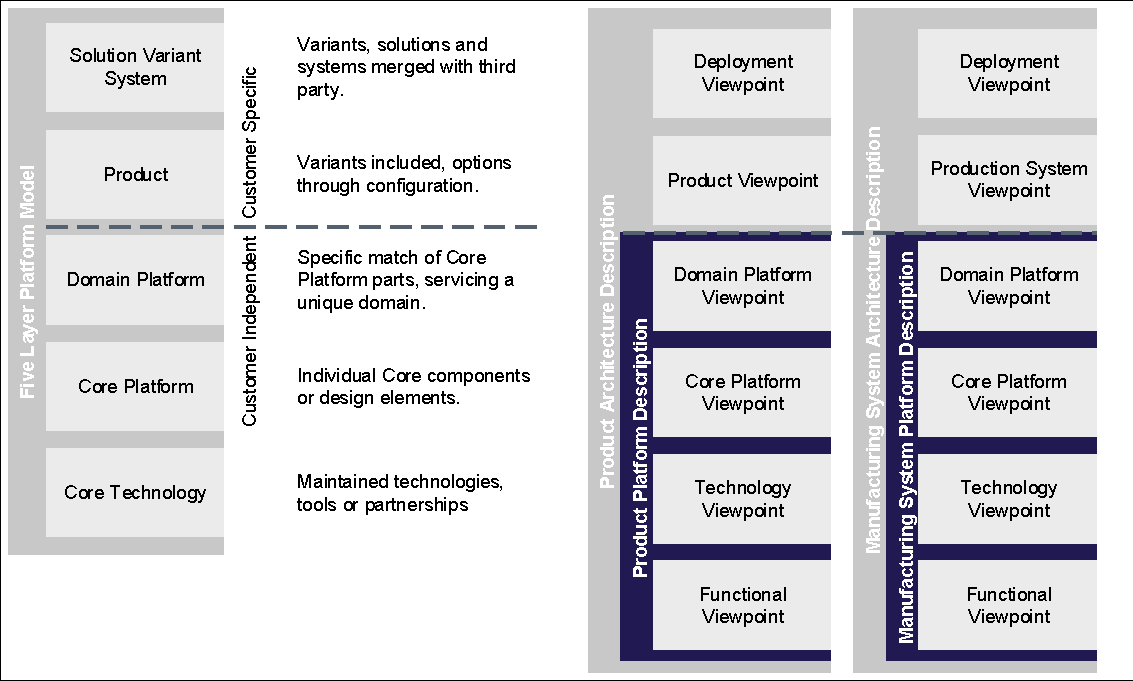
\includegraphics[width=.9\textwidth, trim=2 2 2 2, clip]{mainmatter/researchResults/figures/FLPM.pdf}
  \caption[Five layer product platform model and revised platform model.]
  {Initial five layer product \gls{glos:platform} model from one of the case companies (left) alongside the revised platform model (right) using viewpoints for both product and manufacturing system platforms~\parencite{SorensenMCPC2017}.}\label{fig:FLPM}
\end{figure}
Each of the \gls{glos:view}s resulting from using a corresponding \gls{glos:viewp} can be explained briefly as:
\begin{itemize}
  \item \textbf{Functional view:} functional structure of the manufacturing system, the elements and their primary interactions, interfaces, and responsibilities.
  \item \textbf{Technology view:} fundamental technologies employed by the company, how they are maintained and developed.
  \item \textbf{Core platform view:} available components, design elements, equipment, \etc{} within the platform.
  \item \textbf{Domain platform view:} how core platforms are used within a specific area of application.
  \item \textbf{System view:} the instantiated system developed from an internal development process using available platforms.
  \item \textbf{Deployment view:} deployment and operation of the instantiated system within its immediate environment.
\end{itemize}

\subsubsection*{The Four Loops}
Four Loops of Concern (FLC) is a method guiding the standardisation of tangible and intangible assets for platform development, leaving out the two non-platform viewpoints on \cref{fig:FLPM} (system and deployment).
\begin{figure}[tb]
  \centering
  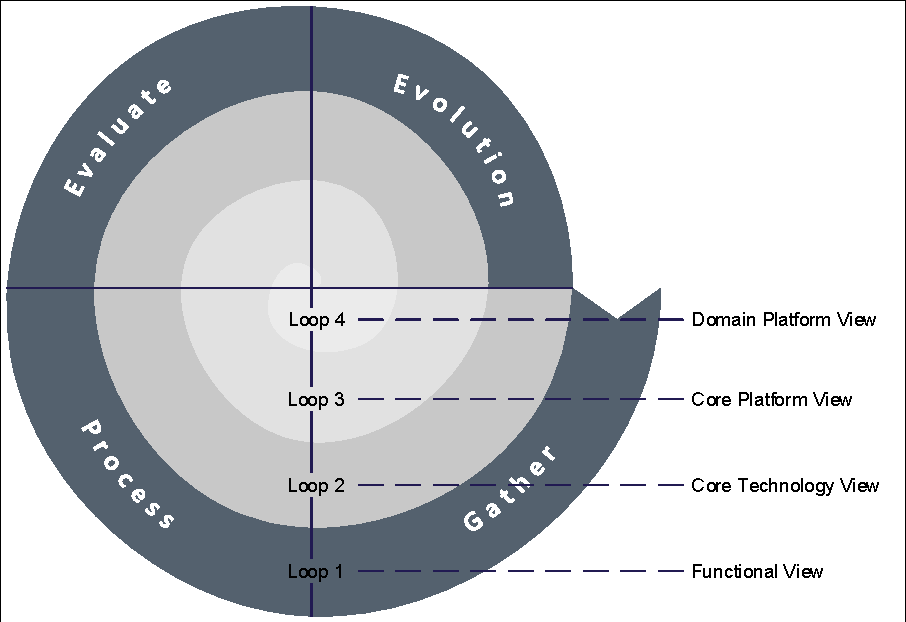
\includegraphics[width=.7\textwidth, trim=2 2 2 2, clip]{mainmatter/researchResults/figures/FLC.pdf}
  \caption[The Four Loops of Concern (FLC) for developing and documenting platforms.]
  {The Four Loops of Concern (FLC) for developing and documenting platforms.
  Redrawn from \parencite{SorensenMCPC2017}.}\label{fig:FLC}
\end{figure}
It consists of four loops, progressing from intangible (functions and technologies) towards tangible (components and instantiations), illustrated as a spiral on \cref{fig:FLC}---a common visual for iterative methods in software development \parencite{Maier2000}.
Each loop consists of four basic steps: 
\begin{enumerate}
  \item \textbf{Gather:} collection of data/information required for a given loop, \eg{} production layouts and schematics. 
  \item \textbf{Process:} application of tools, methods, and models to refine and structure data, \eg{} function-means trees.
  \item \textbf{Evaluate:} synthesis of information based on refined data, \eg{} mapping of functions to technologies.
  \item \textbf{Evolution:} decisions made regarding the next steps in development, \eg{} discontinuation of old technology and implementation of new.
\end{enumerate}
Going through all four steps for all four loops results in the creation of four \gls{glos:view}s describing a platform.
The output for each loop can be summarised as: (loop 1) functional elements and (loop 2) technologies to be supported in the future, (loop 3) a catalogue of platforms (components, equipment and modules), and (loop 4) guidelines on when and how to use specific platforms.
Completing all four loops ensures that a view is created for each \gls{glos:platform} \gls{glos:viewp} shown on \cref{fig:FLPM}.

\subsubsection*{Findings}
FLC was applied in two separate case companies with separate participants.
Both case studies covered one production segment with multiple manufacturing systems.
In both studies, the main sources of information were system experts, ERP systems, and data collected manually from the manufacturing systems.
As a result of applying FLC, a book was created by each company, containing the resulting information and decisions from the platform development process.
The books represent the first iteration of a collection of platform descriptions for each company.
They did not cover all elements identified during the development process in detail, but described them briefly, detailed a smaller number of platforms, and set up guiding principles for future development.

Numerous challenges appeared during the case studies.
Many of these were related to the lack of objective tools and measures for identifying potential platforms and commonality across manufacturing systems.
Most of the available data was based on knowledge from system experts and stakeholders, including design drivers, system characteristics, and functions, making this data subjective in nature.
Specifically, a classification scheme for processes or functions in manufacturing systems would be beneficial to the data gathering phase, and facilitate a more objective comparison of manufacturing system characteristics.
Further, the vocabulary, and need to consider principles rather than moving directly to physical concepts and solutions, proved difficult.
In an effort to accommodate issues with the vocabulary, words like ``\gls{glos:viewp}'' and ``\gls{glos:view}'' were not used in the primary project group, but the concepts remained relevant.

\subsubsection*{Conclusions}
The Four Loops of Concern is an iterative approach to develop and document \gls{glos:platform}s through standardisation of tangible and intangible elements of a system.
It is based on concepts and methods from software architecture development, and has been applied in two separate case studies.
While FLC was applied successfully in both cases, there is a need for more objectivity and for making the method and vocabulary more consistent and easily relatable to developers, designers, and stakeholders.

\subsection{Implications}
The paper summarised above describes the first platform development project within each company, and the first case study of this \PhD{} project. 
As such, it set the stage and direction for much of the research to follow.
During the case study and work on the paper, it became clear that consistent communication and a relatable vocabulary was key to getting designers and developers motivated and involved in the platform development process.
Too many new and foreign concepts were introduced rather quickly during the case study.
The purpose of the development project and the new concepts was not made sufficiently clear early on in the project.
With much of the project relying heavily on subjective information from experts and stakeholders, their individual understanding of these concepts and purposes greatly influenced the outcomes of the case study, and highlighted the need for more consistency, coherency, and objectivity during the development process.
The outcome and contributions of the paper can be summarised as:
\begin{enumerate}
  \item An iterative method to platform development and documentation.
  \item Experiences in platform development added to the knowledge base.
  \item Successful application and an increased understanding of ISO 42010 concepts and tools to advance platform development.
  \item A direction for future research on tools and methods to address the challenges encountered during the project.
\end{enumerate}